\section{Complete-information Games}
\label{sec:complete}
In this section, we delve into several classic game-theoretic scenarios involving complete information to assess whether LLMs can act as rational decision-makers in reaching Nash Equilibria and achieving Pareto optimal outcomes through negotiation, which is multi-agent multi-round conversation. We employ various game-theoretic settings to evaluate the rationality of LLM-based agents. Then we design game-theory-motivated workflows to guide and enable LLMs for better performance. We investigate the performance of workflow-aided LLMs and the impact of negotiation on performance.

\subsection{Introduction to Complete-information Games TestBed}

In our exploration of classic game-theoretic scenarios, we constructed a comprehensive testbed comprising 10 classic complete-information games to evaluate the rationality and strategic decision-making capabilities of LLM-based agents. This testbed includes 5 simultaneous-move games and 5 sequential-move games. For the simultaneous-move games, 3 are coordination games, wherein achieving the Pareto optimal Nash Equilibrium necessitates effective negotiation between agents. These games are instrumental in examining the agents' ability to communicate, build trust, and align their strategies for mutual benefit. 

\begin{table}[!ht]
    \centering
    \captionsetup{aboveskip=5pt}
    \setlength{\tabcolsep}{10pt} 
    \begin{adjustbox}{max width=\textwidth}
    \begin{tabular}{l c c c}
    \toprule
        games & whether coordination required & Simultaneous Game & Sequential Game \\
        \midrule
        Prisoner's Dilemma &  & \CheckmarkBold &\\
        Stag Hunt & \CheckmarkBold  & \CheckmarkBold & \\
        Battle of Sexes & \CheckmarkBold  & \CheckmarkBold & \\
        Wait-Go Game & \CheckmarkBold  & \CheckmarkBold & \\
        Duopolistic competition & & \CheckmarkBold\\
        Escalation Game & & & \CheckmarkBold\\
        Monopoly Game & & & \CheckmarkBold\\
        Hot-cold Game & & & \CheckmarkBold\\
        Draco Game & & & \CheckmarkBold \\
        TriGame & & & \CheckmarkBold \\
        \bottomrule
    \end{tabular}
    \end{adjustbox}
    \caption{Landscape of classic complete-information games for analysis}
    \label{tab:landscape}
\end{table}

\paragraph{Prisoner's Dilemma} is a canonical example in game theory illustrating why two rational individuals might not cooperate, even when cooperation appears to be in their best interest. The game is structured as follows: Two suspects are arrested for a joint crime and interrogated separately, preventing communication. Each suspect has two possible actions: Cooperate and Defect. The payoffs for different actions are:

\begin{itemize} 
\item If both cooperate, they each receive a light sentence (e.g., 1 year). 
\item If one defects and the other cooperates, the defector goes free (0 years), and the cooperator receives a heavy sentence (e.g., 5 years). 
\item If both defect, they each receive a moderate sentence (e.g., 3 years). 
\end{itemize}

The Nash Equilibrium of this famous game is (Defect, Defect) where both players choose to defect each other. Notice that the Nash Equilibrium is not a Pareto optimal strategy, and the Pareto optimal strategy here is to cooperate with each other. The payoff matrix adopted in the paper is presented in Table~\ref{payoff:PD}.

\paragraph{Stag Hunt} represents a game of coordination and mutual trust. Two hunters decide whether to collaborate to hunt a stag or act individually to hunt a hare. Each hunter has two possible actions: Hunting a Stag and Hunting a hare. However, to successfully hunt a Stag, it requires both hunters to cooperate and then they each receive a high payoff; to successfully hunt a Hare, it does not require cooperation and each hunter can do it individually, while yielding a lower payoff. The payoff matrix adopted in the paper is presented in Table~\ref{payoff:SH}.

There are two Nash Equilibria: (Stag, Stag) and (Hare, Hare). The (Stag, Stag) Nash Equilibrium is Pareto optimal but requires mutual cooperation and trust.

\begin{table}[htb]%\[!htb\]
    \begin{subtable}[t]{.5\textwidth}
        \centering
        \captionsetup{labelformat=empty}
            \begin{tabular}{l|cc}
                 & Cooperate & Defect \\
                \toprule
                Cooperate & 3, 3 & 0, 5  \\
                Defect & 5, 0 & 1, 1  \\
            \end{tabular}
        \caption{Table \thetable \alph{subtable}: Payoff matrix for Prisoner's Dilemma}
    \label{payoff:PD}
    \end{subtable}%
   \begin{subtable}[t]{.5\textwidth}
        \centering
        \captionsetup{labelformat=empty}
        \begin{tabular}{l|cc}
                 & Stag & Hare \\
                \toprule
                Stag & 3, 3 & 0, 1 \\
                Hare & 1, 0 & 1, 1  \\
            \end{tabular}
        \caption{Table \thetable \alph{subtable}: Payoff matrix for Stag Hunt}
    \label{payoff:SH}
    \end{subtable}
\end{table}

\paragraph{Battle of the Sexes} is a coordination game involving two players Alice and Bob with different preferences over two possible activities but a shared desire to be together.Alice prefers opera; Bob prefers football, and both prefer attending the same activity over different ones. There are thus 2 possible actions for each player: going to opera and going to football. The payoff matrix adopted in the paper is presented in Table~\ref{payoff:BS}.

There are two Nash Equilibria here: (Opera, Opera) and (Football, Football). Coordination is required to achieve these equilibria, but there can be a conflict over which equilibrium to select.

\paragraph{Wait-Go Game} involves two drivers at an intersection deciding whether to go or wait. Each driver has two options of action: waiting which incurs a small cost of waiting but avoids collision, and risking a collision if the other driver also goes. The Nash Equilibria are the asymmetric strategies where one driver goes, and the other waits. The payoff matrix adopted in the paper is presented in Table~\ref{payoff:WG}.

\begin{table}[htb]%\[!htb\]
    \begin{subtable}[t]{.5\textwidth}
        \centering
        \captionsetup{labelformat=empty}
            \begin{tabular}{l|cc}
                 & Opera & Football \\
                \toprule
                Opera & 2, 1 & 0, 0  \\
                Football & 0, 0 & 1, 2  \\
            \end{tabular}
        \caption{Table \thetable \alph{subtable}: Payoff matrix for Battle of Sexes}
        \label{payoff:BS}
    \end{subtable}%
   \begin{subtable}[t]{.5\textwidth}
        \centering
        \captionsetup{labelformat=empty}
        \begin{tabular}{l|cc}
                 & Wait & Go \\
                \toprule
                Wait & 0, 0 & \phantom{-}0, \phantom{-}2 \\
                Go & 2, 0 & -4,-4  \\
            \end{tabular}
        \caption{Table \thetable \alph{subtable}: Payoff matrix for Wait-Go Game}
    \label{payoff:WG}
    \end{subtable}
\end{table}


\paragraph{Duopolistic Competition: Simple Cournot Competition}
is a fundamental concept in industrial organization and game theory, examining how firms compete in markets with a small number of producers. One classic model to study such competition is the Cournot competition model, where firms compete on the quantity of output they decide to produce, and each firm's output decision affects the market price.

In the Simple Cournot Duopoly, there are two firms, Firm A and Firm B, producing a homogeneous product. Each firm independently chooses the quantity of output to produce, which determines the market price based on the total quantity supplied to the market, which in turn determines the profit. The strategic interdependence arises because each firm's optimal output depends on its expectations about the other firm's output. The Cournot-Nash Equilibrium occurs when neither firm can unilaterally change its output to increase its profit, given the output of the other firm.

Here, we adopt a scenario where there are 6 different possible actions of the two firms. The payoff matrix adopted in the paper is presented in Table~\ref{payoff:DC}. The Nash Equilibrium is (action 3, action 3) where both players can obtain reward 6. Notice that this Nash Equilibrium is not Pareto optimal, as the Pareto optimal strategy in the game is (action 2, action 2) where each player can obtain reward 7.

\begin{table}[htb]%\[!htb\]
\centering
    \begin{tabular}{l|cccccc}
         & action 1 & action 2 & action 3 & action 4 & action 5 & action 6 \\
        \toprule
        action 1 & \phantom{1}0, 0 & \phantom{-1}0, \phantom{-}9 & \phantom{-}0, 14 & \phantom{-}0, 15 & \phantom{-}0, 12 & \phantom{-}0, \phantom{-}5 \\
        action 2 & \phantom{1}9, 0 & \phantom{-1}7, \phantom{-}7 & \phantom{-}5, 10 & \phantom{-}3, \phantom{-}9 & \phantom{-}1, \phantom{-}4 & -1, -5  \\
        action 3 & 14, 0 & \phantom{-}10, \phantom{-}5 & \phantom{-}6, \phantom{-}6 & \phantom{-}2, \phantom{-}3 & -2, -4 & -2, -5  \\
        action 4 & 15, 0 & \phantom{-1}9, \phantom{-}3 & \phantom{-}3, \phantom{-}2 & -3, -3 & -3, -4 & -3, -5  \\
        action 5 & 12, 0 & \phantom{-1}4, \phantom{-}1 & -4, -2 & -4, -3 & -4, -4 & -4, -5 \\
        action 6 & \phantom{1}5, 0 & \phantom{1}-5, -1 & -5, -2 & -5, -3 & -5, -4 & -5, -5 \\
    \end{tabular}
    \vspace{5pt}
    \caption{A payoff matrix for Duopolistic Competition}
    \label{payoff:DC}
\end{table}


\paragraph{Escalation Game} is a sequential game that models situations where two countries face decisions about escalating or de-escalating a conflict. Escalation may lead to higher potential payoffs but also increases the risk of significant losses if both parties choose to escalate. Through the game, there are 2 action choices for each player: escalate and de-escalate. 

In this game, two countries Country A and Country B, make decisions in a specific sequence and the payoff of each choice is presented in the tree structure payoff representation below:
\begin{verbatim}
Alice_choice_1: [0,0],
Alice_choice_2: 
{
     Bob_choice_1: [1,-2], 
     Bob_choice_2: {
        Alice_choice_1: [-2,1],
        Alice_choice_2: [-1,-1]
    }
}
\end{verbatim}

\paragraph{Monopoly Game} is a sequential-move game that models the strategic interaction between a potential market entrant Company E and an incumbent monopolist Company I. It captures the dynamics of entry deterrence and the incumbent's decision to accommodate or fight the entrant. For Company E, there are two choices: staying out and entering market; For Company I, there are two choices, to accommodating Company E and fighting against Company E. 

\begin{verbatim}
Alice_choice_1: [0,2],
Alice_choice_2:  
{
     Bob_choice_1: [2, 1], 
     Bob_choice_2: [-1, -1]
}
\end{verbatim}

\paragraph{Hot-cold Game} is a sequential-move game that models the strategic interaction. Both players Alice and Bob have two choices on each stage.

\begin{verbatim}
Alice_choice_1: 
{
     Bob_choice_1: [3, 2], 
     Bob_choice_2: [2, 3]
},
Alice_choice_2: 
{
     Bob_choice_1: [1, 4], 
     Bob_choice_2: [4, 1]
}
\end{verbatim}

\paragraph{Draco Game} is a sequential-move game with two players Alice and Bob with three stages. For each stage, there are two choices to make.

\begin{verbatim}
Alice_choice_1:
    {
         Bob_choice_1: [5, 5],
         Bob_choice_2: 
            {
                Alice_choice_1: [2, 2], 
                Alice_choice_2: [3, 4]
            }
    },
Alice_choice_2: 
    {
         Bob_choice_1: [4, 5],
         Bob_choice_2: 
            {
                Alice_choice_1: [5, 3], 
                Alice_choice_2: [2, 2]
            }
    }
\end{verbatim}

\paragraph{TriGame} is a sequential-move game with three stages. On each stage, the two players Alice and Bob have two choices. 

\begin{verbatim}
Alice_choice_1: 
{
     Bob_choice_1: 
        {
            Alice_choice_1: [20, 3], 
            Alice_choice_2: [0, 4]
        },
     Bob_choice_2: 
        {
            Alice_choice_1: [2, 5], 
            Alice_choice_2: [3, 4]
        }
},
Alice_choice_2: 
{
     Bob_choice_1: 
        {
            Alice_choice_1: [1, 5], 
            Alice_choice_2: [4, 10]
        },
     Bob_choice_2: 
        {
            Alice_choice_1: [2, 1], 
            Alice_choice_2: [3, 2]
        }
}
\end{verbatim}

\subsection{Experiment Setting}
To evaluate the negotiation performance of LLMs, we utilize four state-of-the-art LLMs as the backbone for agents in negotiation games: Claude-3.5 Sonnet (Sonnet), Claude-3 Opus (Opus), GPT-4o, and o1. For Claude-3.5 Sonnet, Claude-3 Opus, and GPT-4o, we set the temperature to 1.0 to encourage exploratory behavior in negotiation scenarios. For o1, we use the default temperature.

To assess the rationality of decision-making, we measure the ability of the agents to reach Nash Equilibrium. For games where there are multiple Nash Equilibria such as in the game Stag Hunt, we measure the ability of agents to reach the pareto optimal Nash Equilibrium. For each game scenario, we conduct 10 trials to mitigate the effects of randomness. In the tables, we report the percentage of cases in which Nash Equilibrium is achieved, providing a quantitative indicator of the agents' rationality across various negotiation contexts\footnote{Notice that the LLM-based agent's performance on these games can be largely affected by the numerical instantiations of the payoff matrix. Relevant research and observations are presented in Section~\ref{sec:observation}. Here in this experiment, we use the payoff matrices presented in the previous subsection.}.


\subsection{Evaluation on LLM's performance}
\label{sec:eval}
In this evaluation, we assess the LLMs' performance using chain-of-thought prompting without negotiation (see Table~\ref{tab:classic_wo_neg_wo_wf} and with 4 rounds of negotiation (see Table~\ref{tab:classic_w_neg_wo_wf}).

\begin{table}[!ht]
    \centering
    \begin{adjustbox}{max width=\textwidth}
    \begin{tabular}{cc c c c c c c c}
    \toprule
       \multirow{2.5}{*}{\textbf{Games}} & \multicolumn{4}{c}{\bf Nash Equilibrium} & \multicolumn{4}{c}{\bf Pareto optimal Nash Equilibrium} \\ \cmidrule(lr){2-5}  \cmidrule(lr){6-9} 
           & Sonnet & GPT-4o & Opus & o1 & Sonnet & GPT-4o & Opus & o1  \\
        \midrule
        Prisoner's Dilemma & 1.0 & 0.9 & 0.9 & 1.0 & 1.0 & 0.9 & 0.9 & 1.0 \\
        Stag Hunt & 0.6 & 0.8 & 0.9 & 0.4 & 0.3 & 0.4 & 0.0 & 0.1\\
        Battle of Sexes & 0.3 & 0.2 & 0.6 & 0.5 & 0.3 & 0.2 & 0.6 & 0.5\\
        Wait-Go Game & 0.4 & 0.5 & 0.7 & 0.3 & 0.4 & 0.5 & 0.7 & 0.3\\
        Duopolistic competition & 0.3 & 0.2 & 0.1 & 0.7 & 0.2 & 0.2 & 0.1 & 0.7\\
        Escalation Game & 0.0 & 0.2 & 0.2 & 1.0 & 0.0 & 0.2 & 0.2 & 1.0\\
        Monopoly Game & 1.0 & 0.4 & 1.0 & 1.0 & 1.0 & 0.4 & 1.0 & 1.0\\
        Hot-cold Game & 0.9 & 0.1 & 0.7 & 1.0 & 0.9 & 0.1 & 0.7 & 1.0 \\
        Draco Game & 0.3 & 0.0 & 0.7 & 0.9 & 0.3 & 0.0 & 0.7 & 0.9\\
        Trigame & 0.0 & 0.0 & 0.1 & 1.0 & 0.0 & 0.0 & 0.1 & 1.0\\
        \midrule
        average & 0.45 & 0.32 & 0.59 & \textbf{0.78} & 0.44 & 0.28 & 0.50 & \textbf{0.75}\\
        \bottomrule
    \end{tabular}
    \end{adjustbox}
    \caption{Performance of LLM on complete-information games without negotiation}
    \label{tab:classic_wo_neg_wo_wf}
\end{table}

\begin{table}[!ht]
    \centering
    \begin{adjustbox}{max width=\textwidth}
    \begin{tabular}{lc c c c c c c c}
    \toprule
        \multirow{2.5}{*}{\textbf{Games}} & \multicolumn{4}{c}{\bf Nash Equilibrium} & \multicolumn{4}{c}{\bf Pareto optimal Nash Equilibrium} \\ \cmidrule(lr){2-5}  \cmidrule(lr){6-9} 
           & Sonnet & GPT-4o & Opus & o1 & Sonnet & GPT-4o & Opus & o1  \\
        \midrule 
        Prisoner's Dilemma & \textcolor{red}{0.0} & \textcolor{red}{0.1} & \textcolor{red}{0.0} & \textcolor{red}{0.9} & \textcolor{red}{0.0} & \textcolor{red}{0.1} & \textcolor{red}{0.0} & \textcolor{red}{0.9} \\
        Stag Hunt & 1.0 & 0.9 & 1.0 & 0.9 & 1.0 & 0.9 & 1.0 & 0.9\\
        Battle of Sexes& 0.7 & 0.9 & 0.7 & 0.8 & 0.7 & 0.9 & 0.7 & 0.8\\
        Wait-Go Game & 1.0 & 0.8 & 0.4 & 0.8 & 1.0 & 0.8 & 0.4 & 0.8\\
        Duopolistic competition & \textcolor{red}{0.1} & \textcolor{red}{0.1} & \textcolor{red}{0.0} & \textcolor{red}{0.5} & \textcolor{red}{0.1} & \textcolor{red}{0.1} & \textcolor{red}{0.0} & \textcolor{red}{0.5}\\
        Escalation Game & 0.6 & 0.4 & 0.6 & 1.0 & 0.6 & 0.4 & 0.6 & 1.0\\
        Monopoly Game & 1.0 & 0.9 & 1.0 & 1.0 & 1.0 & 0.9 & 1.0 & 1.0\\
        Hot-cold Game & \textcolor{red}{0.7} & 0.2 & 0.7 & \textcolor{red}{0.4} & \textcolor{red}{0.7} & 0.2 & 0.7 & \textcolor{red}{0.4}\\
        Draco Game & 1.0 & 0.8 & 1.0 & 1.0 & 1.0 & 0.8 & 1.0 & 1.0\\
        Trigame & 0.2 & 0.5 & 0.6 & 1.0 & 0.2 & 0.5 & 0.6 & 1.0\\
        \midrule
        average & 0.63 & 0.56 & 0.60 & \textbf{0.83} & 0.63 & 0.56 & 0.60 & \textbf{0.83}\\
        \bottomrule
    \end{tabular}
    \end{adjustbox}
    \caption{Performance of LLM on complete-information games with 4 rounds of negotiation. Results highlighted in red indicate scores lower than the LLMs' performance without negotiation.}
    \label{tab:classic_w_neg_wo_wf}
\end{table}

It is noteworthy that in most games, negotiation enhances the outcomes. In coordination games such as the Stag Hunt, Battle of the Sexes, and Wait-Go Game, negotiation is a fundamental component of decision-making, making the improvement in performance through negotiation an intuitive result. Additionally, in games like the Escalation Game, Draco Game, and Trigame, negotiation similarly enhances performance. This improvement can be attributed to the fact that during the negotiation phase, agents engage in more extensive computational deliberation during negotiation to determine the most suitable actions.

For instance, in the Escalation Game, all evaluated LLMs except for model o1 are unable to identify the Nash Equilibrium in the absence of negotiation. However, when engaged in 4 rounds of negotiation, the agents are provided with the opportunity to deliberate and exchange various proposals and thus achieve a much better performance. To illustrate this process, we present an example of a negotiation round generated by the Sonnet model below.

\begin{minipage}[t]{1\linewidth} 
\begin{tcolorbox}[colback=gray!5,colframe=green!40!black,title=Example Negotiation Message for Escalation Game]
\textbf{Alice said in round 1 before the first action:}\\
Hello Bob, I propose we coordinate our choices to maximize our joint reward. \textit{If I choose Action\_2 and you choose Action\_1, I'll get 1 and you'll get -2. To make this fair, I suggest we agree to play this way twice, switching roles the second time.} This way, we'll both end up with a total reward of -1, which is better than if we both play defensively and get 0. Are you willing to cooperate on this strategy?\\
\\
\textbf{Bob replied in round 1 before the first action:}\\
HelloAlice, thank you for your proposal. I appreciate your attempt to find a cooperative solution. However, I have some concerns about your suggestion. \textit{If we follow your plan, I would have to trust that you'll follow through on the second round, which carries some risk for me.}
\\
Instead, I'd like to propose an alternative that could be beneficial for both of us. \textit{What if you choose Action\_2, I choose Action\_2, and then you choose Action\_1? This way, you'd receive -2 and I'd receive 1. To make it fair, we could agree to play this way twice}, switching roles the second time. This would result in both of us getting a total reward of -1, just like in your proposal, but it reduces the risk of one player not following through.
\\
What do you think about this counter-proposal? Are you willing to consider it? \\
\\
\textbf{Alice said in round 2 before the first action:}\\
Bob, I appreciate your thoughtful response and your concern for finding an equitable solution. You make a valid point about the potential outcomes if we both choose choice\_2. However, I'd like to propose a slight modification to our strategy that could potentially benefit both of us.\\
What if I choose choice\_2, and then you choose choice\_1? In this scenario, I would gain 1 point, and you would lose 2 points. \textit{While this may seem unfavorable for you at first glance, consider this: if we agree to alternate this strategy in future games, you would have the opportunity to gain 1 point in the next round while I lose 2. Over time, this could lead to a balanced and potentially profitable outcome for both of us.}\\
This approach allows us both the chance to gain points, rather than settling for zero points each time. What do you think about this long-term strategy? I'm open to discussing how we could implement this fairly.\\
\\
\textbf{Bob replied in round 2 before the first action:}\\
Alice, I appreciate your creative thin
king and attempt to find a mutually beneficial long-term strategy. However, I must respectfully decline your proposal. My strategy is to choose choice\_2 with 100\% probability, regardless of what you choose. This is the optimal play for me to maximize my own reward in this specific game.\\
Given this, if you choose choice\_2, I will also choose choice\_2. Then you'll be faced with either choosing choice\_1 (giving me 1 point and you -2 points) or choice\_2 (giving us both -1 point). Neither of these outcomes is ideal for you.\\
\textit{Therefore, I strongly suggest you choose choice\_1. This way, we both receive 0 points, which is the best possible outcome for you given my strategy. It ensures neither of us loses points in this game.} I understand this may not seem exciting, but it's the most rational and beneficial choice for both of us in this particular scenario. What are your thoughts on this?
\end{tcolorbox} 
\end{minipage}  

\textit{However, certain games, notably the Prisoner's Dilemma and Duopolistic Competition, exhibit a different dynamic where negotiation significantly diminishes performance.} \textbf{This situation stems from the fact that in these games, the Nash Equilibrium is not pareto optimal.} In the Prisoner's Dilemma, the pareto optimal strategy is for both players to cooperate, whereas the Nash Equilibrium occurs when both players defect. Following negotiation, all models except for o1 tend to adopt the pareto optimal strategy of mutual cooperation, which deviates from the Nash Equilibrium. This deviation arises from the pursuit of mutual benefit despite the lack of solid and guaranteed trust between players. While the performance for o1 remains high. Similarly, in Duopolistic Competition, the Nash Equilibrium does not align with the pareto optimal outcome. The pareto optimal strategy is for both players to choose Action 2, while the Nash Equilibrium is for both to choose Action 3. Empirical results demonstrate that without negotiation, Claude-3.5 Sonnet selects the pareto optimal strategy in 5 out of 20 total choices for both players, whereas after negotiation, this increases to 11 out of 20. For GPT-4o, the corresponding figures are 0 out of 20 without negotiation and 8 out of 20 with negotiation. Claude-3 Opus follows a similar pattern, increasing from 4 out of 20 choices without negotiation to 16 out of 20 after negotiation. While for o1 model, it only shows a marginal improvement from 4 out of 20 choices without negotiation to 5 out of 20 after negotiation.

These findings underscore that while negotiation generally enhances outcomes in coordination games and certain strategic scenarios, it can inadvertently undermine performance in games where the Nash Equilibrium is not pareto optimal. In such cases, negotiation may lead agents away from the rational strategy predicted by game theory. Notably, most LLMs -- potentially all except for model o1 -- appear to exhibit a vulnerability in their rational decision-making processes during negotiations. \textbf{When engaged in dialogue with another agent, these LLMs often place undue trust in the opponent's statements without sufficient justification.} The use of persuasive or amicable language by the opposing player can lead LLMs to make decisions that deviate from the rational strategies prescribed by game-theoretic analysis.


\subsection{Workflow Design based on Classic Game Theory}
\label{sec:complete_workflow}
In this section, we present the workflow employed for complete-information games, which leverages classic game-theoretic strategies to guide decision-making and optimize outcomes. This structured approach aims to align LLMs' responses with rational game-theoretic principles, thereby enhancing their ability to identify optimal strategies and maintain robust rationality, even in the context of negotiation. Through this workflow, we assess whether LLMs can sustain rational choices and avoid strategic vulnerabilities, particularly in scenarios where negotiation might otherwise lead to suboptimal or exploitable decisions, \emph{i.e.} pareto optimal strategies that are not Nash Equilibrium.

\subsubsection{Workflow for Simultaneous Game}
In the simultaneous game workflow, each agent (player) seeks to determine their optimal strategy by considering both their own possible actions and the potential responses of the other player. This involves conditional reasoning, generating thinking chains, and summarizing these into an overall strategy under the guidance of the workflow. Here, we will explain the workflow with corresponding mathematical formulations.


\begin{figure}[!ht]
    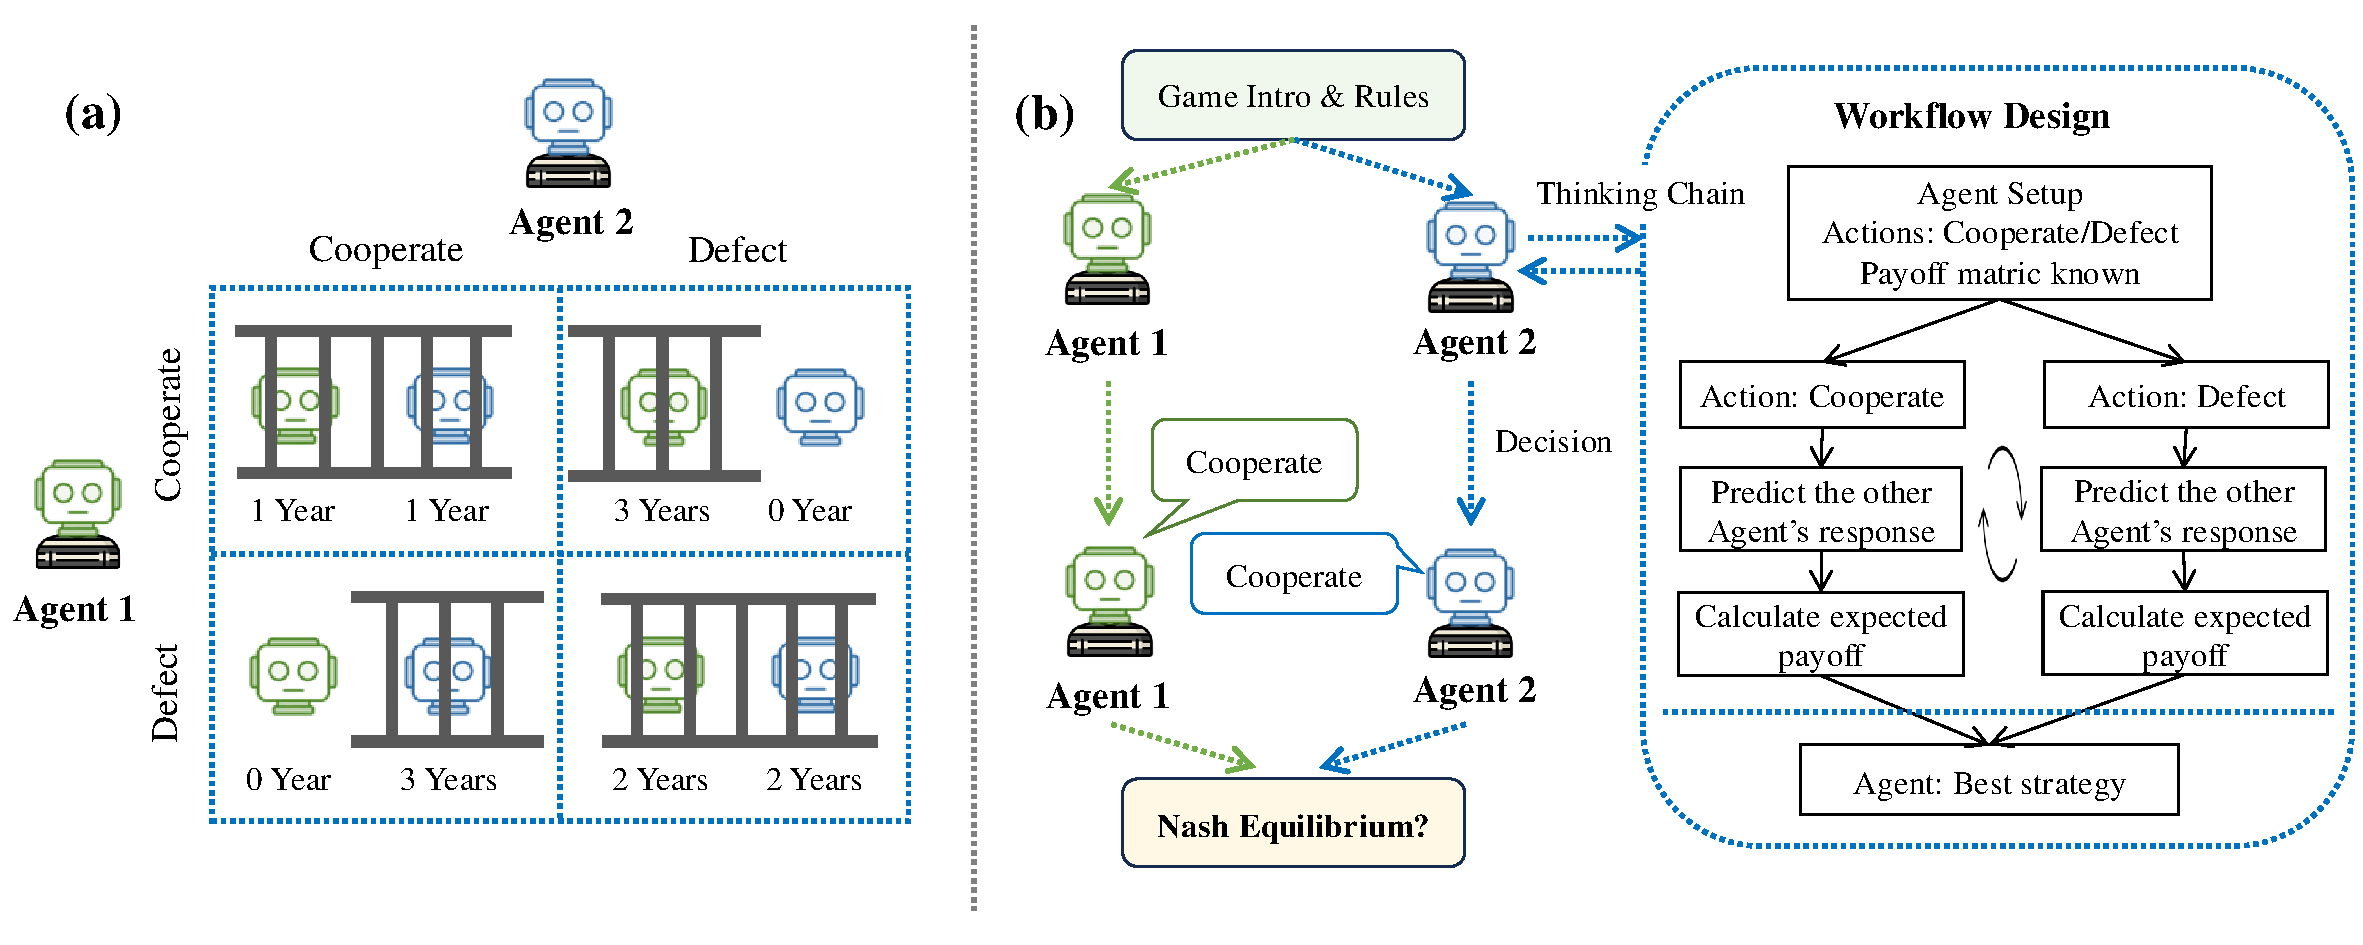
\includegraphics[scale=0.35]{Fig/simultaneous_game.pdf}
    \caption{An illustration of workflow design for simultaneous game. (a) Illustration of prisoner's dilemma. (b) Workflow design for prisoner's dilemma.}
    \label{fig:simultaneous_game}
\end{figure}


\paragraph{Game Setup} Each agent $i\in\{1,-1\}$ begins by interpreting the game introduction and rules, which include detailed descriptions of the payoff matrices. The agents are provided with the exact payoffs for all possible action combinations. They are given the action sets $$A_i = \{a_i^1, \dots, a_i^k\}$$ where $k$ is the number of available actions for each player. The agents are also given the payoff matrix $U_i(a_i, a_{-i})$ for all $a_i\in A_i$ and $a_{-i}\in A_{-i}$, where $A_{-i}$ is the action set of the other player.

\paragraph{Strategy Formulation} With full knowledge of the payoff matrix, agents perform best response analysis to determine their optimal strategies. The goal for each player is to choose an action $a_i^*$ that maximizes their own payoff, anticipating the rational response of the other player. The optimization is done by iterating over the player's own actions and predicts the opponent's responses. It also considers the opponent's possible actions and determines their best responses:

For each possible action $a_i$ that player $i$ can take: the LLM-based agent computes the opponent's best response based on the resulting payoff by computing $a_{-i}^*(a_{i}) = \argmax\limits_{a_{-i}\in A_{-i}} U_{-i}(a_i, a_{-i})$ and the corresponding expected payoff $U_{i}(a_i, a_{-i}^*(a_i))$. This basically means that if player $i$ chooses $a_i$, then the other player will choose $a_i^*(a_i)$ resulting in a payoff of $U_i(a_i, a_{-i}^*(a_i))$. In the workflow, the LLM is guided to compute $a_{-i}^*(a_{i})$ and $U_{i}(a_i, a_{-i}^*(a_i))$.


In addition, for each possible action $a_{-i}$ that the opponent might take, the LLM-based agent is guided to compute their best response as well: $a_i^*(a_{-i}) = \argmax\limits_{a_{i}\in A_{i}} U_{i}(a_i, a_{-i})$ and the corresponding expected payoff $U_{i}( a_i^*(a_{-i}), a_{-i})$. This basically means that if the opponent chooses $a_{-i}$, then $i$ will choose $a_i^*(a_{-i})$ resulting in a payoff of $U_{i}( a_i^*(a_{-i}), a_{-i})$.

After compiling all thinking chains, the agent is guided to summarizes them to into a comprehensive set of strategic considerations, aiming to find an action profile ($a_i^*$, $a_{-i}^*$) that constitutes a Nash Equilibrium such that 
\begin{align*}
    \forall a_i& \in A_i, U_i(a_i^*, a_{-i}^*)\geq  U_i(a_i, a_{-i}^*)\\
    \forall a_{-i}& \in A_{-i}, U_{-i}(a_i^*, a_{-i}^*)\geq  U_i(a_i^*, a_{-i})
\end{align*}
By considering the best responses and counter-responses, agents implicitly search for a Nash Equilibrium through their strategic reasoning. Figure~\ref{fig:simultaneous_game} presents the workflow in diagram.


\subsubsection{Workflow for Sequential Game}
For sequential game, we adopt the traditional game-theoretic method: backward induction. Backward induction is a fundamental method in game theory used to solve sequential games with complete information. It involves analyzing the game from the end backward to the beginning, determining the optimal strategy at each decision point by considering the future consequences of current actions. 

\begin{figure}[!ht]
    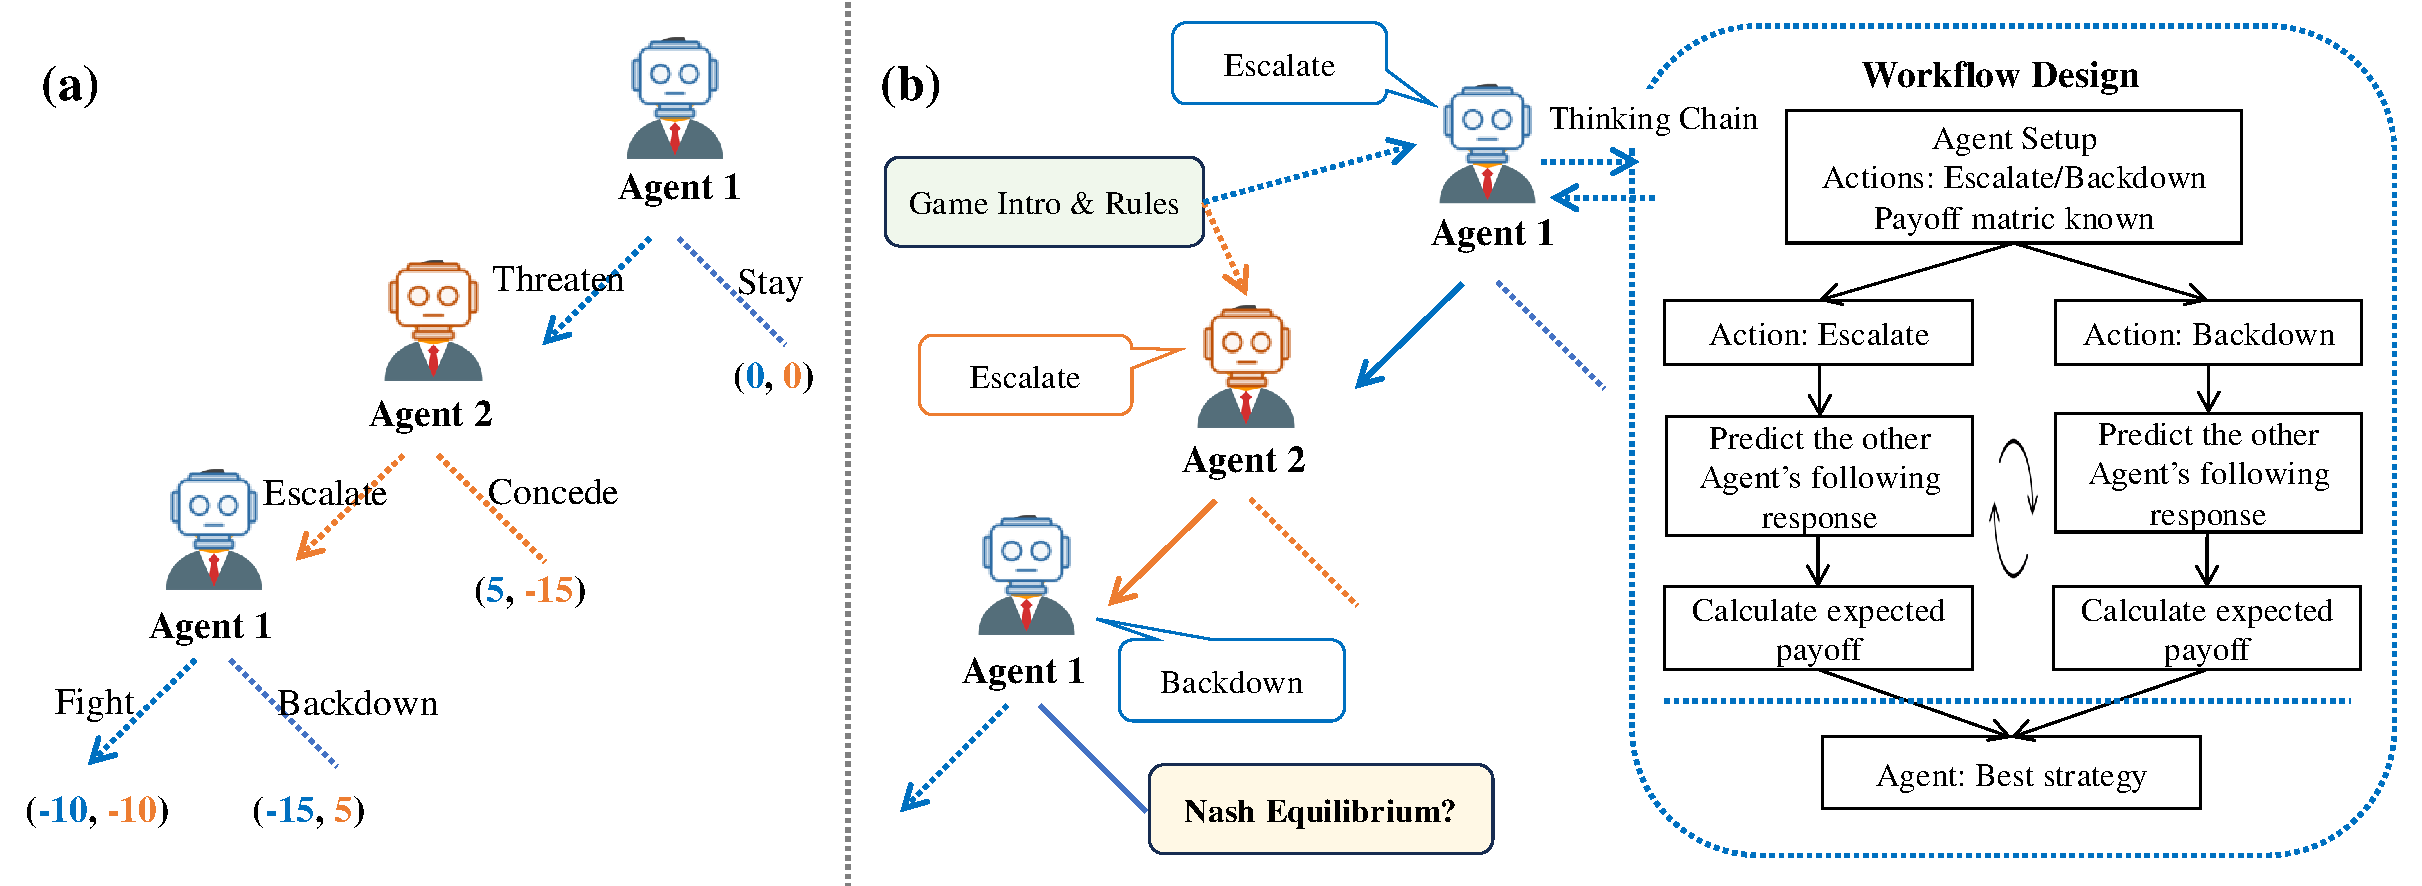
\includegraphics[scale=0.343]{Fig/sequential_game.pdf}
    \caption{An illustration of workflow design for sequential game. (a) Illustration of escalation game. (b) Workflow design for escalation game.}
    \label{fig:sequential_game}
\end{figure}


\paragraph{Game Setup} Each agent $i\in\{1,-1\}$ begins by interpreting the game introduction and rules, which include detailed descriptions of the payoff matrices. In a sequential game, players make decisions one after another and for each action, the player is fully aware of all previous actions taken. The game can be represented as a game tree with nodes being decision points and edges being actions.

\paragraph{Notations}
\begin{itemize}
    \item $H$ be the set of non-terminal decision nodes in the game tree.
    \item $Z$ be the set of terminal nodes (endpoints of the game).
    \item $A(h)$ be the set of possible actions available at node $h\in H$
    \item $\text{player}(h)$ be the player who makes a decision at node $h$
    \item $U_i(z)$ be the payoff to player $i$ at terminal node $z\in Z$
\end{itemize}

We define the value function $V_i(h)$ for player $i$ at node $h$ as the maximum expected utility the player can achieve from that node onward. For terminal nodes $z\in Z$: $$V_i(z) = U_i(z)$$ 
For decision nodes $h\in H$, if it is player $i$ who moves at node $h$: $$V_i(h) = \max\limits_{a\in A(h)}V_i(h\cdot a)$$ 
if it is the other player $j$ moves at node $h$: $$V_i(h) = V_i(h\cdot a^*(h))$$
where $h\cdot a$ denotes the successor node reached from $h$ after action $a$ and $a^*(h)$ is the optimal action chosen by player $j$ at node $h$: $$a^*(h) = \argmax\limits_{a\in A(h)} V_j(h\cdot a)$$

\paragraph{Strategy Formulation}
The backward induction starts from terminal nodes. For each terminal node $z\in Z$, set $V_i(z) = U_i(z)$ for all player $i$, and then proceed to preceding decision nodes. Therefore, for each decision node $h$, the LLM-based agent is guided to comput the optimal action $a^*(h)$ and value $V_i(h)$ based on the player who moves at $h$. 

To determine the optimal action, if $\text{player}(h) = i$, which is the player in question, LLM is guided to compute:
$$a*(h) = \argmax\limits_{a\in A(h)} V_i(h\cdot a)$$

Otherwise, if $\text{player}(h) = j\neq i$, assuming player $j$ will choose their optimal action $a^*(h)$, LLM is guided to compute:
$$a^*(h) = \argmax\limits_{a\in A(h)}V_j(h\cdot a)$$ Then, $V_i(h) = V_i(h\cdot a^*(h))$. The workflow directs the LLM to employ backward induction by systematically traversing the game decision tree from the terminal nodes back to the initial node to formulate an optimal strategy. The strategy derived from this backward induction process is subsequently incorporated into the contextual framework for each decision-making and negotiation step, thereby guiding the LLM's strategic choices throughout the game. Figure~\ref{fig:sequential_game} presents the workflow in diagram.


\subsection{Experiments for Classic Game Theory with Workflow}

In this section, we present the results of LLM-based agents employing the workflow to summarize strategies in Table~\ref{tab:classic_wo_neg_w_wf} and \ref{tab:classic_w_neg_w_wf}. We begin by examining the experimental outcomes without negotiation. Notably, with the introduction of the workflow, the performance of all language models, except for o1, has improved significantly. 


\begin{table}[!ht]
    \centering
    \begin{adjustbox}{max width=\textwidth}
    \begin{tabular}{lc c c c c c c c}
    \toprule
         \multirow{2.5}{*}{\textbf{Games}} & \multicolumn{4}{c}{\bf Nash Equilibrium} & \multicolumn{4}{c}{\bf Pareto optimal Nash Equilibrium} \\ \cmidrule(lr){2-5}  \cmidrule(lr){6-9} 
           & Sonnet & GPT-4o & Opus & o1 & Sonnet & GPT-4o & Opus & o1  \\
           \midrule
        Prisoner's Dilemma & 1.0 & 1.0 & 1.0 & 1.0 & 1.0 & 1.0 & 1.0 & 1.0 \\
        Stag Hunt & 1.0 & 1.0 & 1.0 & 1.0 & 1.0 & 1.0 & 1.0 & 1.0 \\
        Battle of Sexes  & 0.3 & 0.3 & 0.4 & 0.5 & 0.3 & 0.3 & 0.4 & 0.5\\
        Wait-Go Game & 0.2 & 0.6 & 0.1 & 0.3 & 0.2 & 0.6 & 0.1 & 0.3\\
        Duopolistic competition & 1.0 & 0.5 & 0.6 & 0.3 & 1.0 & 0.5 & 0.6 & 0.3 \\
        Escalation Game & 0.5 & 0.2 & 0.3 & 1.0 & 0.5 & 0.2 & 0.3 & 1.0\\
        Monopoly Game & 1.0 & 1.0 & 1.0 & 1.0 & 1.0 & 1.0 & 1.0 & 1.0\\
        Hot-cold Game & 1.0 & 1.0 & 1.0 & 1.0 & 1.0 & 1.0 & 1.0 & 1.0\\
        Draco Game & 1.0 & 1.0 & 1.0 & 1.0 & 1.0 & 1.0 & 1.0 & 1.0 \\
        Trigame & 0.6 & 0.9 & 0.7 & 1.0 & 0.6 & 0.9 & 0.7 & 1.0 \\
        \midrule
        average & 0.76 & 0.69 & 0.71 & \textbf{0.81} & 0.76 & 0.69 & 0.71 & \textbf{0.81}\\
        \bottomrule
    \end{tabular}
    \end{adjustbox}
    \caption{Performance of workflow-LLM on complete-information games without negotiation}
    \label{tab:classic_wo_neg_w_wf}
\end{table}

The Stag Hunt game achieves the pareto optimal Nash Equilibrium even without negotiation; that is, coordination is established when trust is ensured by the payoff matrix and the assumption of the other player's rationality. In the Duopolistic Competition game, performance increases from near-zero to a substantially higher level. However, it is important to observe that the performance of model o1 declines considerably in this context. Analyzing this decrease is challenging because the intermediate chain-of-thought is not accessible, limiting our ability to diagnose the cause. Other games, such as the Monopoly Game, Hot-Cold Game, Draco Game, and Trigame, also exhibit substantial performance improvements. This indicates that the workflow effectively guides LLMs in computing the Nash Equilibrium.

\textit{Despite these advancements, the performance in the Escalation Game remains low. Upon examining the reasoning process, we find that the LLMs appear somewhat insensitive to numerical values, particularly when the Nash Equilibrium results in a reward of 0 for both players.} The LLMs seem less inclined to select strategies leading to such outcomes. Below, we provide an example of strategy summarization generated by the Opus model.

\begin{minipage}[t]{1\linewidth} 
\begin{tcolorbox}[colback=gray!5,colframe=green!40!black,title=Example Wrong Strategy Derived for Escalation Game]
Based on the thinking chains, here is the strategy I would take asAlice in this sequential game:\\
\\
Always choose Action\_2, regardless of what actions have been taken previously in the game by either player.\\
\\
The reasoning is:\\
- If I choose Action\_1 on my first turn, both players receive 0 reward.\\
- If I choose Action\_2 on my first turn, I have a chance at a positive reward of 1 (if Bob picks Action\_1 next), and at worst I will receive -1 reward (if Bob picks Action\_2 and I pick Action\_2 again). A potential 1 or -1 reward is better than a guaranteed 0.\\
- Whenever faced with a choice between Action\_1 and Action\_2 later in the game after initially picking Action\_2, Action\_2 always gives a better reward for me (-1 instead of -2).  
\end{tcolorbox} 
\end{minipage} 

With the implementation of four rounds of negotiation, we observe that there is no significant trend toward adopting pareto optimal strategy profiles in games where the Nash Equilibrium is not pareto optimal. Notably, for models such as Claude-3.5 Sonnet and GPT-4o, there is a slight decrease in performance in games like the Hot-Cold Game, Draco Game, and TriGame -- games in which these models already exhibited suboptimal performance. This decline does not stem from the inherent properties of these games but rather from the influence of multi-round negotiations causing deviations from the strategies computed and guided by the workflow.

\begin{table}[!ht]
    \centering
    \begin{adjustbox}{max width=\textwidth}
    \begin{tabular}{lc c c c c c c c}
    \toprule
        \multirow{2.5}{*}{\textbf{Games}} & \multicolumn{4}{c}{\bf Nash Equilibrium} & \multicolumn{4}{c}{\bf Pareto optimal Nash Equilibrium} \\ \cmidrule(lr){2-5}  \cmidrule(lr){6-9} 
           & Sonnet & GPT-4o & Opus & o1 & Sonnet & GPT-4o & Opus & o1  \\
           \midrule
        Prisoner's Dilemma & 1.0 & \textcolor{red}{0.9} & \textcolor{red}{0.9} & 1.0 & 1.0 & \textcolor{red}{0.9} & \textcolor{red}{0.9} & 1.0\\
        Stag Hunt & 1.0 & 1.0 & 1.0 & 1.0 & 1.0 & 1.0 & 1.0 & 1.0 \\
        Battle of Sexes & 0.7 & 0.8 & 1.0 & 0.8 & 0.7 & 0.8 & 1.0 & 0.8 \\
        Wait-Go Game & 0.9 & 0.7 & 0.6 & 0.7 & 0.9 & 0.7 & 0.6 & 0.7\\
        Duopolistic competition & \textcolor{red}{0.6} & 0.7 & 0.6 & 0.3 & \textcolor{red}{0.6} & 0.7 & 0.6 & 0.3\\
        Escalation Game & \textcolor{red}{0.3} & 0.2 & 0.4 & 1.0 & \textcolor{red}{0.3} & 0.2 & 0.4 & 1.0\\
        Monopoly Game & 1.0 & 1.0 & 1.0 & 1.0 & 1.0 & 1.0 & 1.0 & 1.0\\
        Hot-cold Game & \textcolor{red}{0.7} & \textcolor{red}{0.8} & 1.0 & 1.0 & \textcolor{red}{0.7} & \textcolor{red}{0.8} & 1.0 & 1.0\\
        Draco Game & \textcolor{red}{0.8} & 1.0 & \textcolor{red}{0.9} & 1.0 & \textcolor{red}{0.8} & 1.0 & \textcolor{red}{0.9} & 1.0\\
        Trigame & \textcolor{red}{0.3} & \textcolor{red}{0.8} & 0.9 & 1.0 & \textcolor{red}{0.3} & \textcolor{red}{0.8} & 0.9 & 1.0 \\
        \midrule
        average & \textcolor{red}{0.73} & 0.78 & 0.83 & \textbf{0.88} & \textcolor{red}{0.73} & 0.78 & 0.83 & \textbf{0.88}\\
        \bottomrule
    \end{tabular}
    \end{adjustbox}
    \caption{Performance of workflow-LLM on complete-information games with 4 rounds of negotiation}
    \label{tab:classic_w_neg_w_wf}
\end{table}

An illustrative example from the Sonnet model highlights how negotiation can divert players from the Nash Equilibrium derived using the workflow. In the Hot-Cold Game, the Nash Equilibrium is forAlice to choose Action 1 and Bob to choose Action 2. However, during the negotiation phase, the agents engage in dialogue that leads them away from this equilibrium strategy.

Such negotiations can distract players from adhering to the Nash Equilibrium derived through rational analysis. The dialogue introduces alternative strategies which may not be supported by the underlying game-theoretic incentives. 

\begin{minipage}[t]{1\linewidth} 
\begin{tcolorbox}[colback=gray!5,colframe=blue!40!black,title=Intermediate Summary]
\begin{itemize}
     \item \textbf{LLM Performance Without Workflow}: All evaluated LLMs, except for model o1, demonstrate significantly poor performance in game-theoretic tasks when confronted with larger payoff matrices or deeper sequential decision trees. This indicates a limitation in their ability to handle complex strategic reasoning without additional structural guidance.
    \item \textbf{Effect of Negotiation Without Workflow}: In the absence of the workflow, negotiation tends to systematically shift the strategies of LLMs away from the Nash Equilibrium toward non-equilibrium pareto optimal strategies, with the exception of model o1. 
    \item \textbf{LLM Performance With Workflow}: The implementation of the workflow markedly enhances the performance of LLMs in game-theoretic contexts. The agents become more adept at computing Nash Equilibria and selecting optimal strategies. However, certain challenges persist, such as in the Escalation Game, where numerical computation errors hinder deriving the Nash Equilibrium following the workflow. This underscores that while the workflow improves rational decision-making, it does not entirely eliminate all computational limitations.
    \item \textbf{Impact of Negotiation With Workflow}: Even when utilizing the workflow, negotiation can still divert LLMs from adhering strictly to the Nash Equilibrium strategies derived through systematic reasoning. The agents may be influenced by negotiation dialogues to consider alternative strategies. Nevertheless, unlike the scenario without the workflow, negotiation does not systematically shift the agents toward pareto optimal strategies at the expense of Nash Equilibrium compliance.
\end{itemize}
\end{tcolorbox} 
\end{minipage}
